\chapter{恒星脉动}
\section{脉动星}
由于恒星在演化过程中会发生膨胀和收缩,这些都是恒星内部维持平衡而产生的过程,这些膨胀和收缩导致的是恒星气体发生运动,形成一种类似驻波的周期性脉动,使恒星的半径发生周期性变化,进而导致光度发生周期性变化。

形象来看,这种波动在恒星内部以声速$v_s=\sqrt{\gamma P/\rho}$来回传播,可以想象,对于半径越大的恒星,其光度越强,波动传播时间越长,脉动周期就越长,这种\textbf{脉动恒星的周光关系}最早被哈佛大学的列维特所发现,计算也可以得到周期和密度的关系:
\begin{equation}
  \Pi\approx\sqrt{3\pi \over 2\gamma G\rho}
\end{equation}

\begin{figure}[hbt]
  \centering
  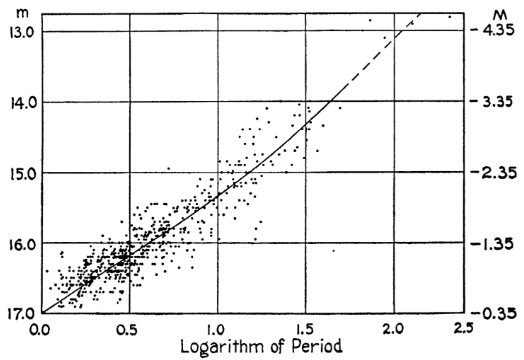
\includegraphics[width=8cm]{chapters/14/cepheid}
  \caption{经典造父变星的周光关系}
  \label{}
\end{figure}

恒星的膨胀和收缩是为了平衡引力,因此正常情况下恒星能够通过这种方式会恢复平衡,而不会演化成周期性的脉动,但是如果有些特殊机制,阻碍其有效平衡引力,就会维持这种膨胀和收缩,形成脉动。

在恒星的绝大部分区域,压缩会使温度升高,不透明度下降;而在\textbf{部分电离区},压缩时一部分压缩功会用于电离,令粒子数密度增加,不透明度反而上升。这会令从内部传播出来的光子无法有效通过,能量会在这里积累,温度上升,又会导致膨胀;同样,膨胀时温度降低,不透明度降低,同时离子结合放出的光子很容易逃离,带走能量,又回导致压缩,形成新的循环。这种不透明度导致脉动的机制被称为\textbf{$\kappa$机制}。

同时,因为部分电离区的压缩会引起电离,因此这里的温度上升程度比周围小,会引起周围的热量向这边传递,这会增强$\kappa$机制,而这种效应被称为\textbf{$\gamma$机制}。

部分电离区在脉动中的作用就像一个弹簧,在恒星膨胀和收缩过程中通过电离和结合的形式吸收和释放能量,维持住脉动。

脉动星在脉动时,会有不同的波动模式,有径向波动和非径向的波动,根据波动模式不同可以将脉动星分为不同类别,并在赫罗图中有对应的不同\textbf{脉动带}区域,当恒星演化到相应区域时会产生相应的脉动,如图\ref{fig:pusating}。

而有些人认为脉动带远不止这些,而我们的太阳就处于一种一条内,由于脉动周期在3-8分钟之间,因此被称为\textbf{五分钟振荡}。

\begin{figure}[hbt]
  \centering
  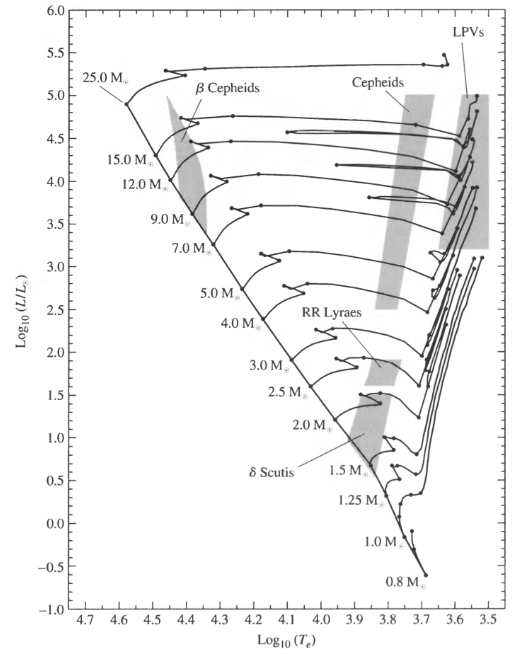
\includegraphics[width=10cm]{chapters/14/pusating}
  \caption{赫罗图上的脉动带}
  \label{fig:pusating}
\end{figure}
